% Kursliste am Desktop (blaues Design, Kategorie Metals aufgeklappt) – Vektor-Nachbau.
% Grundlage: DOM-Messung originals/messungen/kursliste-desktop.json (CSS-px, Fenster
% 2040 x 986 wie bei bar.tex). Bild = der gemessene Block .quote-list, 304 x 410 px.
% Koordinaten unten in CSS-px, y nach unten, Ursprung = linke obere Ecke des Blocks.
%
% Gemessen:
%   Block              304 x 410, Fläche rgb(4,39,60) (= Seitenhintergrund), Inter
%   button.quotes-ttl  x0, je 304 x 28, padding 0 20px 0 0, text-align left,
%                      Inter 500, 12 px / line-height 14 px, weiß, Fläche = Block;
%                      y Forex 0, Stocks 32, Cryptos 64, Indices 96, Energies 128,
%                      Metals 160 (aufgeklappt, margin-bottom 4 px), Commodities 350,
%                      ETFs 382
%     Pfeil auf/ab     NICHT gemessen (kein Knoten, kein ::after) – WEGGELASSEN
%   li > a (Zeile)     x0, 304 x 30, y 192 / 224 / 256, padding 6px 8px, Radius 3 px,
%                      Fläche rgba(14,80,114,0.1), Inter 400, 12 px / line-height 18 px
%     i.icon-star      x8 y+8 14 x 14, icomoon 14 px, U+E916, rgb(91,106,130)
%                      – nur, wenn icons.tikz \iconstar enthält (derzeit nicht; die Font
%                      liegt nicht im Repo), sonst leer
%     img              x33,3 (Palladium x30,8) y+8,5, 22 x 14 (27 x 14)
%                      – WEGGELASSEN (Rasterbild), die Fläche bleibt leer
%     span.arrow       NICHT gemessen – WEGGELASSEN
%     span.symbol      x73,6 y+6, 63,15 x 18: Copper, Gold, Palladium (weiß)
%     Kurse (2 Spalten) x145,2 und x210,9, Textbox y+6,8, 15,2 hoch; Farbe Copper
%                      rgb(255,255,255) (color00), Gold und Palladium rgb(83,188,81)
%                      (color-green-main)
%     i.icon-information x278,6 y+8,5, 14 x 14, icomoon 14 px, U+E93A, rgb(34,100,134)
%                      -> \iconinfo aus icons.tikz
%   Zwischen Palladium (Unterkante 286) und Commodities (350) liegen 64 px, für die die
%   Messung keine Knoten enthält (vermutlich Platinum und Silver, nicht belegt): die
%   Fläche bleibt leer.
%
% Grundlinien (wie bar.tex): Oberkante der Textbox + Ascent 12 px (Chrome rundet Ascent/
% Descent in Gerätepixeln: 12 + 3,2 = 15,2 px). Zeilen: Textbox y+6,8 gemessen -> y+18,8.
% Schaltflächen: Zeile (14 px) mittig in 28 px -> Oberkante 7, Textbox 0,8 px darüber
% (wie bar.tex bei 14 px) -> Grundlinie y+18,2.
% Icons: Glyphenbox (Ascent 960 + Descent 64 = 1 em) = Box des <i>, 14 x 14 px.
%
% Abweichung vom Original (Regeln des Nutzers): keine Zahlen, kein Bid/Ask -> beide Kurse
% heißen „Kurs“, in den gemessenen Farben. Die Instrumentnamen bleiben.
%
% Marken (Schalter \ifmarken, Standard: an; ohne Marken bauen mit
%   xelatex -jobname=kursliste-desktop-ohne '\def\ohnemarken{}% Kursliste am Desktop (blaues Design, Kategorie Metals aufgeklappt) – Vektor-Nachbau.
% Grundlage: DOM-Messung originals/messungen/kursliste-desktop.json (CSS-px, Fenster
% 2040 x 986 wie bei bar.tex). Bild = der gemessene Block .quote-list, 304 x 410 px.
% Koordinaten unten in CSS-px, y nach unten, Ursprung = linke obere Ecke des Blocks.
%
% Gemessen:
%   Block              304 x 410, Fläche rgb(4,39,60) (= Seitenhintergrund), Inter
%   button.quotes-ttl  x0, je 304 x 28, padding 0 20px 0 0, text-align left,
%                      Inter 500, 12 px / line-height 14 px, weiß, Fläche = Block;
%                      y Forex 0, Stocks 32, Cryptos 64, Indices 96, Energies 128,
%                      Metals 160 (aufgeklappt, margin-bottom 4 px), Commodities 350,
%                      ETFs 382
%     Pfeil auf/ab     NICHT gemessen (kein Knoten, kein ::after) – WEGGELASSEN
%   li > a (Zeile)     x0, 304 x 30, y 192 / 224 / 256, padding 6px 8px, Radius 3 px,
%                      Fläche rgba(14,80,114,0.1), Inter 400, 12 px / line-height 18 px
%     i.icon-star      x8 y+8 14 x 14, icomoon 14 px, U+E916, rgb(91,106,130)
%                      – nur, wenn icons.tikz \iconstar enthält (derzeit nicht; die Font
%                      liegt nicht im Repo), sonst leer
%     img              x33,3 (Palladium x30,8) y+8,5, 22 x 14 (27 x 14)
%                      – WEGGELASSEN (Rasterbild), die Fläche bleibt leer
%     span.arrow       NICHT gemessen – WEGGELASSEN
%     span.symbol      x73,6 y+6, 63,15 x 18: Copper, Gold, Palladium (weiß)
%     Kurse (2 Spalten) x145,2 und x210,9, Textbox y+6,8, 15,2 hoch; Farbe Copper
%                      rgb(255,255,255) (color00), Gold und Palladium rgb(83,188,81)
%                      (color-green-main)
%     i.icon-information x278,6 y+8,5, 14 x 14, icomoon 14 px, U+E93A, rgb(34,100,134)
%                      -> \iconinfo aus icons.tikz
%   Zwischen Palladium (Unterkante 286) und Commodities (350) liegen 64 px, für die die
%   Messung keine Knoten enthält (vermutlich Platinum und Silver, nicht belegt): die
%   Fläche bleibt leer.
%
% Grundlinien (wie bar.tex): Oberkante der Textbox + Ascent 12 px (Chrome rundet Ascent/
% Descent in Gerätepixeln: 12 + 3,2 = 15,2 px). Zeilen: Textbox y+6,8 gemessen -> y+18,8.
% Schaltflächen: Zeile (14 px) mittig in 28 px -> Oberkante 7, Textbox 0,8 px darüber
% (wie bar.tex bei 14 px) -> Grundlinie y+18,2.
% Icons: Glyphenbox (Ascent 960 + Descent 64 = 1 em) = Box des <i>, 14 x 14 px.
%
% Abweichung vom Original (Regeln des Nutzers): keine Zahlen, kein Bid/Ask -> beide Kurse
% heißen „Kurs“, in den gemessenen Farben. Die Instrumentnamen bleiben.
%
% Marken (Schalter \ifmarken, Standard: an; ohne Marken bauen mit
%   xelatex -jobname=kursliste-desktop-ohne '\def\ohnemarken{}% Kursliste am Desktop (blaues Design, Kategorie Metals aufgeklappt) – Vektor-Nachbau.
% Grundlage: DOM-Messung originals/messungen/kursliste-desktop.json (CSS-px, Fenster
% 2040 x 986 wie bei bar.tex). Bild = der gemessene Block .quote-list, 304 x 410 px.
% Koordinaten unten in CSS-px, y nach unten, Ursprung = linke obere Ecke des Blocks.
%
% Gemessen:
%   Block              304 x 410, Fläche rgb(4,39,60) (= Seitenhintergrund), Inter
%   button.quotes-ttl  x0, je 304 x 28, padding 0 20px 0 0, text-align left,
%                      Inter 500, 12 px / line-height 14 px, weiß, Fläche = Block;
%                      y Forex 0, Stocks 32, Cryptos 64, Indices 96, Energies 128,
%                      Metals 160 (aufgeklappt, margin-bottom 4 px), Commodities 350,
%                      ETFs 382
%     Pfeil auf/ab     NICHT gemessen (kein Knoten, kein ::after) – WEGGELASSEN
%   li > a (Zeile)     x0, 304 x 30, y 192 / 224 / 256, padding 6px 8px, Radius 3 px,
%                      Fläche rgba(14,80,114,0.1), Inter 400, 12 px / line-height 18 px
%     i.icon-star      x8 y+8 14 x 14, icomoon 14 px, U+E916, rgb(91,106,130)
%                      – nur, wenn icons.tikz \iconstar enthält (derzeit nicht; die Font
%                      liegt nicht im Repo), sonst leer
%     img              x33,3 (Palladium x30,8) y+8,5, 22 x 14 (27 x 14)
%                      – WEGGELASSEN (Rasterbild), die Fläche bleibt leer
%     span.arrow       NICHT gemessen – WEGGELASSEN
%     span.symbol      x73,6 y+6, 63,15 x 18: Copper, Gold, Palladium (weiß)
%     Kurse (2 Spalten) x145,2 und x210,9, Textbox y+6,8, 15,2 hoch; Farbe Copper
%                      rgb(255,255,255) (color00), Gold und Palladium rgb(83,188,81)
%                      (color-green-main)
%     i.icon-information x278,6 y+8,5, 14 x 14, icomoon 14 px, U+E93A, rgb(34,100,134)
%                      -> \iconinfo aus icons.tikz
%   Zwischen Palladium (Unterkante 286) und Commodities (350) liegen 64 px, für die die
%   Messung keine Knoten enthält (vermutlich Platinum und Silver, nicht belegt): die
%   Fläche bleibt leer.
%
% Grundlinien (wie bar.tex): Oberkante der Textbox + Ascent 12 px (Chrome rundet Ascent/
% Descent in Gerätepixeln: 12 + 3,2 = 15,2 px). Zeilen: Textbox y+6,8 gemessen -> y+18,8.
% Schaltflächen: Zeile (14 px) mittig in 28 px -> Oberkante 7, Textbox 0,8 px darüber
% (wie bar.tex bei 14 px) -> Grundlinie y+18,2.
% Icons: Glyphenbox (Ascent 960 + Descent 64 = 1 em) = Box des <i>, 14 x 14 px.
%
% Abweichung vom Original (Regeln des Nutzers): keine Zahlen, kein Bid/Ask -> beide Kurse
% heißen „Kurs“, in den gemessenen Farben. Die Instrumentnamen bleiben.
%
% Marken (Schalter \ifmarken, Standard: an; ohne Marken bauen mit
%   xelatex -jobname=kursliste-desktop-ohne '\def\ohnemarken{}% Kursliste am Desktop (blaues Design, Kategorie Metals aufgeklappt) – Vektor-Nachbau.
% Grundlage: DOM-Messung originals/messungen/kursliste-desktop.json (CSS-px, Fenster
% 2040 x 986 wie bei bar.tex). Bild = der gemessene Block .quote-list, 304 x 410 px.
% Koordinaten unten in CSS-px, y nach unten, Ursprung = linke obere Ecke des Blocks.
%
% Gemessen:
%   Block              304 x 410, Fläche rgb(4,39,60) (= Seitenhintergrund), Inter
%   button.quotes-ttl  x0, je 304 x 28, padding 0 20px 0 0, text-align left,
%                      Inter 500, 12 px / line-height 14 px, weiß, Fläche = Block;
%                      y Forex 0, Stocks 32, Cryptos 64, Indices 96, Energies 128,
%                      Metals 160 (aufgeklappt, margin-bottom 4 px), Commodities 350,
%                      ETFs 382
%     Pfeil auf/ab     NICHT gemessen (kein Knoten, kein ::after) – WEGGELASSEN
%   li > a (Zeile)     x0, 304 x 30, y 192 / 224 / 256, padding 6px 8px, Radius 3 px,
%                      Fläche rgba(14,80,114,0.1), Inter 400, 12 px / line-height 18 px
%     i.icon-star      x8 y+8 14 x 14, icomoon 14 px, U+E916, rgb(91,106,130)
%                      – nur, wenn icons.tikz \iconstar enthält (derzeit nicht; die Font
%                      liegt nicht im Repo), sonst leer
%     img              x33,3 (Palladium x30,8) y+8,5, 22 x 14 (27 x 14)
%                      – WEGGELASSEN (Rasterbild), die Fläche bleibt leer
%     span.arrow       NICHT gemessen – WEGGELASSEN
%     span.symbol      x73,6 y+6, 63,15 x 18: Copper, Gold, Palladium (weiß)
%     Kurse (2 Spalten) x145,2 und x210,9, Textbox y+6,8, 15,2 hoch; Farbe Copper
%                      rgb(255,255,255) (color00), Gold und Palladium rgb(83,188,81)
%                      (color-green-main)
%     i.icon-information x278,6 y+8,5, 14 x 14, icomoon 14 px, U+E93A, rgb(34,100,134)
%                      -> \iconinfo aus icons.tikz
%   Zwischen Palladium (Unterkante 286) und Commodities (350) liegen 64 px, für die die
%   Messung keine Knoten enthält (vermutlich Platinum und Silver, nicht belegt): die
%   Fläche bleibt leer.
%
% Grundlinien (wie bar.tex): Oberkante der Textbox + Ascent 12 px (Chrome rundet Ascent/
% Descent in Gerätepixeln: 12 + 3,2 = 15,2 px). Zeilen: Textbox y+6,8 gemessen -> y+18,8.
% Schaltflächen: Zeile (14 px) mittig in 28 px -> Oberkante 7, Textbox 0,8 px darüber
% (wie bar.tex bei 14 px) -> Grundlinie y+18,2.
% Icons: Glyphenbox (Ascent 960 + Descent 64 = 1 em) = Box des <i>, 14 x 14 px.
%
% Abweichung vom Original (Regeln des Nutzers): keine Zahlen, kein Bid/Ask -> beide Kurse
% heißen „Kurs“, in den gemessenen Farben. Die Instrumentnamen bleiben.
%
% Marken (Schalter \ifmarken, Standard: an; ohne Marken bauen mit
%   xelatex -jobname=kursliste-desktop-ohne '\def\ohnemarken{}\input{kursliste-desktop}'):
% Stil der Nummern in panel.pdf (weißer Kreis 22 px, Ziffer Inter 600 12 px in #04273C,
% Grundlinie 4 px unter der Mitte); 1 links neben dem Info-Zeichen der Zeile Gold (3 px
% Abstand, mittig zum Zeichen).
\documentclass[border=0pt]{standalone}
\usepackage{fontspec}
\usepackage{tikz}
\setmainfont{Inter}% Inter 4.0 (Paket fonts-inter), wie bar.tex
\newfontfamily\mittel{Inter Medium}%     button.quotes-ttl, font-weight 500
\newfontfamily\halbfett{Inter SemiBold}% Ziffern der Marken (wie panel.pdf)

\newlength\px \setlength\px{0.75bp}% 1 CSS-px
\newcommand\schrift{\fontsize{9bp}{10.5bp}\selectfont}% 12 px
\definecolor{seite}{RGB}{4,39,60}%      Block und Schaltflächen
% Zeile: rgba(14,80,114,0.1) über rgb(4,39,60) = (5,0; 43,1; 65,4) -> rgb(5,43,65)
\definecolor{zeile}{RGB}{5,43,65}%
\definecolor{stern}{RGB}{91,106,130}%   i.icon-star
\definecolor{info}{RGB}{34,100,134}%    i.icon-information
\definecolor{gruen}{RGB}{83,188,81}%    color-green-main
\definecolor{markenziffer}{HTML}{04273C}% Ziffer der Marken (wie panel.pdf)
\input{icons.tikz}

\newif\ifmarken \markentrue
\ifdefined\ohnemarken \markenfalse\fi

% \kategorie{<y>}{<Name>}
\newcommand\kategorie[2]{%
  \node[anchor=base west,inner sep=0,outer sep=0,text=white,font=\schrift\mittel]
    at (0,#1+18.2) {#2};}

% \icon{<x>}{<y Oberkante>}{<Farbe>}{<Icon>}: Box 14 x 14 px (icons.tikz: 24 px, y nach oben)
\newcommand\icon[4]{%
  \begin{scope}[shift={(#1,#2+14)},x=0.4375bp,y=0.4375bp,color=#3]#4\end{scope}}% 14/24 px

% \instrument{<y>}{<Name>}{<Farbe der Kurse>}
\newcommand\instrument[3]{%
  \fill[zeile,rounded corners=3\px] (0,#1) rectangle (304,#1+30);
  \ifdefined\iconstar \icon{8}{#1+8}{stern}{\iconstar}\fi
  \node[anchor=base west,inner sep=0,outer sep=0,text=white] at (73.6,#1+18.8) {#2};
  \node[anchor=base west,inner sep=0,outer sep=0,text=#3] at (145.2,#1+18.8) {Kurs};
  \node[anchor=base west,inner sep=0,outer sep=0,text=#3] at (210.9,#1+18.8) {Kurs};
  \icon{278.6}{#1+8.5}{info}{\iconinfo}}

% \marke{<y Mitte>}{<Nummer>}: Kreis 22 px, 3 px links vor dem Info-Zeichen (x 278,6)
\newcommand\marke[2]{%
  \fill[white] (264.6,#1) circle[radius=11];
  \node[anchor=base,inner sep=0,outer sep=0,text=markenziffer,
    font=\schrift\halbfett] at (264.6,#1+4) {#2};}

\begin{document}%
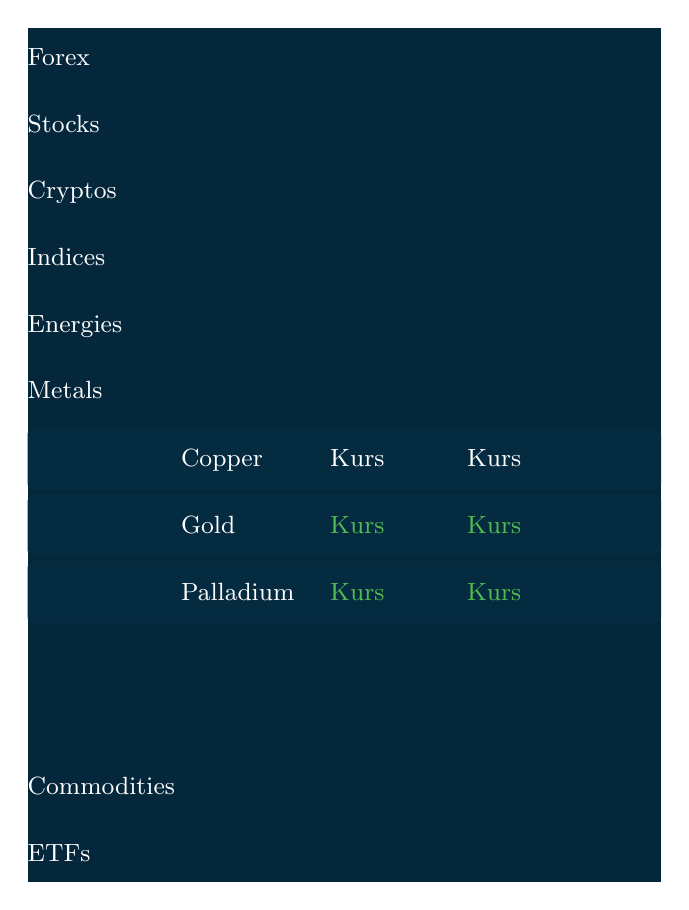
\begin{tikzpicture}[x=\px,y={(0,-\px)},font=\schrift]
  \path[use as bounding box] (0,0) rectangle (304,410);
  \fill[seite] (0,0) rectangle (304,410);
  \kategorie{0}{Forex}
  \kategorie{32}{Stocks}
  \kategorie{64}{Cryptos}
  \kategorie{96}{Indices}
  \kategorie{128}{Energies}
  \kategorie{160}{Metals}
  \instrument{192}{Copper}{white}
  \instrument{224}{Gold}{gruen}
  \instrument{256}{Palladium}{gruen}
  \kategorie{350}{Commodities}
  \kategorie{382}{ETFs}
  \ifmarken
    \marke{224+8.5+7}{1}
  \fi
\end{tikzpicture}%
\end{document}
'):
% Stil der Nummern in panel.pdf (weißer Kreis 22 px, Ziffer Inter 600 12 px in #04273C,
% Grundlinie 4 px unter der Mitte); 1 links neben dem Info-Zeichen der Zeile Gold (3 px
% Abstand, mittig zum Zeichen).
\documentclass[border=0pt]{standalone}
\usepackage{fontspec}
\usepackage{tikz}
\setmainfont{Inter}% Inter 4.0 (Paket fonts-inter), wie bar.tex
\newfontfamily\mittel{Inter Medium}%     button.quotes-ttl, font-weight 500
\newfontfamily\halbfett{Inter SemiBold}% Ziffern der Marken (wie panel.pdf)

\newlength\px \setlength\px{0.75bp}% 1 CSS-px
\newcommand\schrift{\fontsize{9bp}{10.5bp}\selectfont}% 12 px
\definecolor{seite}{RGB}{4,39,60}%      Block und Schaltflächen
% Zeile: rgba(14,80,114,0.1) über rgb(4,39,60) = (5,0; 43,1; 65,4) -> rgb(5,43,65)
\definecolor{zeile}{RGB}{5,43,65}%
\definecolor{stern}{RGB}{91,106,130}%   i.icon-star
\definecolor{info}{RGB}{34,100,134}%    i.icon-information
\definecolor{gruen}{RGB}{83,188,81}%    color-green-main
\definecolor{markenziffer}{HTML}{04273C}% Ziffer der Marken (wie panel.pdf)
% Icons als TikZ-Pfade – erzeugt von tools/icons_aus_font.py, nicht von Hand ändern.
% Schrift: 230d1684-icomoon-1-icomoon.b9abfeda36b81d3e.ttf (icomoon, Version 1.0, TrueType), sha256 951e3a5eca89112f…
% Herkunft: Webfont „icomoon“ der Plattform (icomoon.b9abfeda36b81d3e.ttf; icomoon.47a83e5a26e26197.woff hat dieselben Tabellen und Glyphen), vom Nutzer hochgeladen am 02.10.2026. Die Schriftdateien liegen NICHT im Repo (Lizenz unklar), nur diese Pfade.
% unitsPerEm 1024; Metriken hhea: Ascent 960, Descent -64.
% Box wie das <i>-Element im Browser: font-size 24px, line-height 24px
% -> Box 24 x 24 px, Ursprung unten links, y nach oben;
%    Grundlinie 1.500 px über der Boxunterkante. 1 Einheit = 1 CSS-px.
% Füllregel nonzero (wie im Browser). Farbe kommt von außen (color=…).
% Gebrauch: \begin{scope}[shift={(<x>,<y>)},x=\px,y=\px,color=<Farbe>]\iconbell\end{scope}

% U+E938 uniE938 – icon-notifications (Glocke); Vorschub 24.000 px; Umriss x 1.99–22.01, y 1.99–22.01 px; 3 Kontur(en)
\newcommand\iconbell{\fill[nonzero rule]
    (19.992,7.711) -- (22.008,7.711) -- (22.008,5.812) -- (1.992,5.812) -- (1.992,7.711) -- (4.008,7.711) -- (4.008,14.391) .. controls (4.008,15.391) and (4.211,16.359) .. (4.617,17.297) .. controls (5.023,18.234) and (5.602,19.055) .. (6.352,19.758) .. controls (7.102,20.477) and (7.965,21.031) .. (8.941,21.422) .. controls (9.918,21.812) and (10.938,22.008) .. (12,22.008) .. controls (13.062,22.008) and (14.082,21.812) .. (15.059,21.422) .. controls (16.035,21.031) and (16.898,20.477) .. (17.648,19.758) .. controls (18.398,19.055) and (18.977,18.234) .. (19.383,17.297) .. controls (19.789,16.359) and (19.992,15.391) .. (19.992,14.391) -- (19.992,7.711) -- cycle
    (18,7.711) -- (18,14.391) .. controls (18,15.141) and (17.848,15.867) .. (17.543,16.57) .. controls (17.238,17.273) and (16.805,17.891) .. (16.242,18.422) .. controls (15.68,18.953) and (15.031,19.363) .. (14.297,19.652) .. controls (13.562,19.941) and (12.797,20.086) .. (12,20.086) .. controls (11.203,20.086) and (10.438,19.941) .. (9.703,19.652) .. controls (8.969,19.363) and (8.32,18.953) .. (7.758,18.422) .. controls (7.195,17.891) and (6.762,17.273) .. (6.457,16.57) .. controls (6.152,15.867) and (6,15.141) .. (6,14.391) -- (6,7.711) -- cycle
    (9,3.891) -- (15,3.891) -- (15,1.992) -- (9,1.992) -- cycle;}

% U+E937 uniE937 – icon-settings (Zahnrad); Vorschub 24.000 px; Umriss x 2.37–21.63, y 1.99–22.01 px; 4 Kontur(en)
\newcommand\icongear{\fill[nonzero rule]
    (3.352,7.008) .. controls (3.133,7.367) and (2.941,7.742) .. (2.777,8.133) .. controls (2.613,8.523) and (2.477,8.922) .. (2.367,9.328) .. controls (2.617,9.453) and (2.844,9.609) .. (3.047,9.797) .. controls (3.25,9.984) and (3.422,10.195) .. (3.562,10.43) .. controls (3.703,10.664) and (3.812,10.914) .. (3.891,11.18) .. controls (3.969,11.445) and (4.008,11.719) .. (4.008,12) .. controls (4.008,12.281) and (3.969,12.555) .. (3.891,12.82) .. controls (3.812,13.086) and (3.703,13.336) .. (3.562,13.57) .. controls (3.422,13.805) and (3.25,14.016) .. (3.047,14.203) .. controls (2.844,14.391) and (2.617,14.547) .. (2.367,14.672) .. controls (2.586,15.484) and (2.91,16.258) .. (3.34,16.992) .. controls (3.77,17.727) and (4.281,18.398) .. (4.875,19.008) .. controls (5.094,18.852) and (5.336,18.734) .. (5.602,18.656) .. controls (5.867,18.578) and (6.141,18.531) .. (6.422,18.516) .. controls (6.703,18.516) and (6.977,18.551) .. (7.242,18.621) .. controls (7.508,18.691) and (7.758,18.797) .. (7.992,18.938) .. controls (8.242,19.062) and (8.461,19.227) .. (8.648,19.43) .. controls (8.836,19.633) and (9,19.852) .. (9.141,20.086) .. controls (9.266,20.336) and (9.359,20.594) .. (9.422,20.859) .. controls (9.484,21.125) and (9.508,21.398) .. (9.492,21.68) .. controls (10.32,21.898) and (11.156,22.008) .. (12,22.008) .. controls (12.844,22.008) and (13.68,21.898) .. (14.508,21.68) .. controls (14.492,21.398) and (14.516,21.125) .. (14.578,20.859) .. controls (14.641,20.594) and (14.734,20.336) .. (14.859,20.086) .. controls (15,19.852) and (15.164,19.633) .. (15.352,19.43) .. controls (15.539,19.227) and (15.758,19.062) .. (16.008,18.938) .. controls (16.242,18.797) and (16.492,18.691) .. (16.758,18.621) .. controls (17.023,18.551) and (17.297,18.516) .. (17.578,18.516) .. controls (17.859,18.531) and (18.133,18.578) .. (18.398,18.656) .. controls (18.664,18.734) and (18.906,18.852) .. (19.125,19.008) .. controls (19.422,18.711) and (19.699,18.395) .. (19.957,18.059) .. controls (20.215,17.723) and (20.445,17.367) .. (20.648,16.992) .. controls (20.867,16.617) and (21.059,16.238) .. (21.223,15.855) .. controls (21.387,15.473) and (21.523,15.078) .. (21.633,14.672) .. controls (21.383,14.547) and (21.156,14.391) .. (20.953,14.203) .. controls (20.75,14.016) and (20.578,13.805) .. (20.438,13.57) .. controls (20.297,13.336) and (20.188,13.086) .. (20.109,12.82) .. controls (20.031,12.555) and (19.992,12.281) .. (19.992,12) .. controls (19.992,11.719) and (20.031,11.445) .. (20.109,11.18) .. controls (20.188,10.914) and (20.297,10.664) .. (20.438,10.43) .. controls (20.578,10.195) and (20.75,9.984) .. (20.953,9.797) .. controls (21.156,9.609) and (21.383,9.453) .. (21.633,9.328) .. controls (21.414,8.516) and (21.09,7.742) .. (20.66,7.008) .. controls (20.23,6.273) and (19.719,5.602) .. (19.125,4.992) .. controls (18.906,5.148) and (18.664,5.266) .. (18.398,5.344) .. controls (18.133,5.422) and (17.859,5.469) .. (17.578,5.484) .. controls (17.297,5.484) and (17.023,5.449) .. (16.758,5.379) .. controls (16.492,5.309) and (16.242,5.203) .. (16.008,5.062) .. controls (15.758,4.938) and (15.539,4.773) .. (15.352,4.57) .. controls (15.164,4.367) and (15,4.148) .. (14.859,3.914) .. controls (14.734,3.664) and (14.641,3.406) .. (14.578,3.141) .. controls (14.516,2.875) and (14.492,2.602) .. (14.508,2.32) .. controls (13.68,2.102) and (12.844,1.992) .. (12,1.992) .. controls (11.156,1.992) and (10.32,2.102) .. (9.492,2.32) .. controls (9.508,2.602) and (9.484,2.875) .. (9.422,3.141) .. controls (9.359,3.406) and (9.266,3.664) .. (9.141,3.914) .. controls (9,4.148) and (8.836,4.367) .. (8.648,4.57) .. controls (8.461,4.773) and (8.242,4.938) .. (7.992,5.062) .. controls (7.758,5.203) and (7.508,5.309) .. (7.242,5.379) .. controls (6.977,5.449) and (6.703,5.484) .. (6.422,5.484) .. controls (6.141,5.469) and (5.867,5.422) .. (5.602,5.344) .. controls (5.336,5.266) and (5.094,5.148) .. (4.875,4.992) .. controls (4.578,5.289) and (4.301,5.605) .. (4.043,5.941) .. controls (3.785,6.277) and (3.555,6.633) .. (3.352,7.008) -- cycle
    (9,6.797) .. controls (9.531,6.5) and (9.992,6.113) .. (10.383,5.637) .. controls (10.773,5.16) and (11.062,4.625) .. (11.25,4.031) .. controls (11.5,4.016) and (11.75,4.008) .. (12,4.008) .. controls (12.25,4.008) and (12.5,4.016) .. (12.75,4.031) .. controls (12.938,4.609) and (13.227,5.141) .. (13.617,5.625) .. controls (14.008,6.109) and (14.469,6.5) .. (15,6.797) .. controls (15.531,7.109) and (16.102,7.312) .. (16.711,7.406) .. controls (17.32,7.5) and (17.922,7.484) .. (18.516,7.359) .. controls (18.672,7.562) and (18.812,7.773) .. (18.938,7.992) .. controls (19.062,8.211) and (19.172,8.438) .. (19.266,8.672) .. controls (18.859,9.125) and (18.547,9.641) .. (18.328,10.219) .. controls (18.109,10.797) and (18,11.391) .. (18,12) .. controls (18,12.625) and (18.113,13.227) .. (18.34,13.805) .. controls (18.566,14.383) and (18.875,14.891) .. (19.266,15.328) .. controls (19.172,15.562) and (19.062,15.789) .. (18.938,16.008) .. controls (18.812,16.227) and (18.672,16.438) .. (18.516,16.641) .. controls (17.922,16.516) and (17.32,16.5) .. (16.711,16.594) .. controls (16.102,16.688) and (15.531,16.891) .. (15,17.203) .. controls (14.469,17.5) and (14.008,17.887) .. (13.617,18.363) .. controls (13.227,18.84) and (12.938,19.375) .. (12.75,19.969) .. controls (12.5,19.984) and (12.25,19.992) .. (12,19.992) .. controls (11.75,19.992) and (11.5,19.984) .. (11.25,19.969) .. controls (11.062,19.391) and (10.773,18.859) .. (10.383,18.375) .. controls (9.992,17.891) and (9.531,17.5) .. (9,17.203) .. controls (8.469,16.891) and (7.898,16.688) .. (7.289,16.594) .. controls (6.68,16.5) and (6.078,16.516) .. (5.484,16.641) .. controls (5.328,16.438) and (5.188,16.227) .. (5.062,16.008) .. controls (4.938,15.789) and (4.828,15.562) .. (4.734,15.328) .. controls (5.141,14.875) and (5.453,14.359) .. (5.672,13.781) .. controls (5.891,13.203) and (6,12.609) .. (6,12) .. controls (6,11.375) and (5.887,10.773) .. (5.66,10.195) .. controls (5.434,9.617) and (5.125,9.109) .. (4.734,8.672) .. controls (4.828,8.438) and (4.938,8.211) .. (5.062,7.992) .. controls (5.188,7.773) and (5.328,7.562) .. (5.484,7.359) .. controls (6.078,7.484) and (6.68,7.5) .. (7.289,7.406) .. controls (7.898,7.312) and (8.469,7.109) .. (9,6.797) -- cycle
    (12,9) .. controls (11.609,9) and (11.227,9.074) .. (10.852,9.223) .. controls (10.477,9.371) and (10.148,9.586) .. (9.867,9.867) .. controls (9.586,10.148) and (9.371,10.477) .. (9.223,10.852) .. controls (9.074,11.227) and (9,11.609) .. (9,12) .. controls (9,12.391) and (9.074,12.773) .. (9.223,13.148) .. controls (9.371,13.523) and (9.586,13.852) .. (9.867,14.133) .. controls (10.148,14.414) and (10.477,14.629) .. (10.852,14.777) .. controls (11.227,14.926) and (11.609,15) .. (12,15) .. controls (12.391,15) and (12.773,14.926) .. (13.148,14.777) .. controls (13.523,14.629) and (13.852,14.414) .. (14.133,14.133) .. controls (14.414,13.852) and (14.629,13.523) .. (14.777,13.148) .. controls (14.926,12.773) and (15,12.391) .. (15,12) .. controls (15,11.609) and (14.926,11.227) .. (14.777,10.852) .. controls (14.629,10.477) and (14.414,10.148) .. (14.133,9.867) .. controls (13.852,9.586) and (13.523,9.371) .. (13.148,9.223) .. controls (12.773,9.074) and (12.391,9) .. (12,9) -- cycle
    (12,10.992) .. controls (12.125,10.992) and (12.25,11.02) .. (12.375,11.074) .. controls (12.5,11.129) and (12.609,11.203) .. (12.703,11.297) .. controls (12.797,11.391) and (12.871,11.5) .. (12.926,11.625) .. controls (12.98,11.75) and (13.008,11.875) .. (13.008,12) .. controls (13.008,12.125) and (12.98,12.25) .. (12.926,12.375) .. controls (12.871,12.5) and (12.797,12.609) .. (12.703,12.703) .. controls (12.609,12.797) and (12.5,12.871) .. (12.375,12.926) .. controls (12.25,12.98) and (12.125,13.008) .. (12,13.008) .. controls (11.875,13.008) and (11.75,12.98) .. (11.625,12.926) .. controls (11.5,12.871) and (11.391,12.797) .. (11.297,12.703) .. controls (11.203,12.609) and (11.129,12.5) .. (11.074,12.375) .. controls (11.02,12.25) and (10.992,12.125) .. (10.992,12) .. controls (10.992,11.875) and (11.02,11.75) .. (11.074,11.625) .. controls (11.129,11.5) and (11.203,11.391) .. (11.297,11.297) .. controls (11.391,11.203) and (11.5,11.129) .. (11.625,11.074) .. controls (11.75,11.02) and (11.875,10.992) .. (12,10.992) -- cycle;}

% U+E90C uniE90C – icon-orders (Liste mit Plus); Vorschub 24.000 px; Umriss x 3.00–21.00, y 1.01–19.99 px; 4 Kontur(en)
\newcommand\iconorders{\fill[nonzero rule]
    (18,9) -- (18,6) -- (21,6) -- (21,4.008) -- (18,4.008) -- (18,1.008) -- (16.008,1.008) -- (16.008,4.008) -- (13.008,4.008) -- (13.008,6) -- (16.008,6) -- (16.008,9) -- cycle
    (10.992,6) -- (10.992,4.008) -- (3,4.008) -- (3,6) -- cycle
    (21,13.008) -- (21,10.992) -- (3,10.992) -- (3,13.008) -- (21,13.008) -- cycle
    (21,19.992) -- (21,18) -- (3,18) -- (3,19.992) -- cycle;}

% U+E93A uniE93A – icon-information (Kreis mit i); Vorschub 24.000 px; Umriss x 1.99–22.01, y 1.99–22.01 px; 4 Kontur(en)
\newcommand\iconinfo{\fill[nonzero rule]
    (12,1.992) .. controls (10.625,1.992) and (9.328,2.258) .. (8.109,2.789) .. controls (6.891,3.305) and (5.828,4.016) .. (4.922,4.922) .. controls (4.016,5.828) and (3.305,6.891) .. (2.789,8.109) .. controls (2.258,9.328) and (1.992,10.625) .. (1.992,12) .. controls (1.992,13.375) and (2.258,14.672) .. (2.789,15.891) .. controls (3.305,17.109) and (4.016,18.172) .. (4.922,19.078) .. controls (5.828,19.984) and (6.891,20.695) .. (8.109,21.211) .. controls (9.328,21.742) and (10.625,22.008) .. (12,22.008) .. controls (13.375,22.008) and (14.672,21.742) .. (15.891,21.211) .. controls (17.109,20.695) and (18.172,19.984) .. (19.078,19.078) .. controls (19.984,18.172) and (20.695,17.109) .. (21.211,15.891) .. controls (21.742,14.672) and (22.008,13.375) .. (22.008,12) .. controls (22.008,10.625) and (21.742,9.328) .. (21.211,8.109) .. controls (20.695,6.891) and (19.984,5.828) .. (19.078,4.922) .. controls (18.172,4.016) and (17.109,3.305) .. (15.891,2.789) .. controls (14.672,2.258) and (13.375,1.992) .. (12,1.992) -- cycle
    (12,4.008) .. controls (13.062,4.008) and (14.082,4.211) .. (15.059,4.617) .. controls (16.035,5.023) and (16.898,5.602) .. (17.648,6.352) .. controls (18.398,7.102) and (18.977,7.965) .. (19.383,8.941) .. controls (19.789,9.918) and (19.992,10.938) .. (19.992,12) .. controls (19.992,13.062) and (19.789,14.082) .. (19.383,15.059) .. controls (18.977,16.035) and (18.398,16.898) .. (17.648,17.648) .. controls (16.898,18.398) and (16.035,18.977) .. (15.059,19.383) .. controls (14.082,19.789) and (13.062,19.992) .. (12,19.992) .. controls (10.938,19.992) and (9.918,19.789) .. (8.941,19.383) .. controls (7.965,18.977) and (7.102,18.398) .. (6.352,17.648) .. controls (5.602,16.898) and (5.023,16.035) .. (4.617,15.059) .. controls (4.211,14.082) and (4.008,13.062) .. (4.008,12) .. controls (4.008,10.938) and (4.211,9.918) .. (4.617,8.941) .. controls (5.023,7.965) and (5.602,7.102) .. (6.352,6.352) .. controls (7.102,5.602) and (7.965,5.023) .. (8.941,4.617) .. controls (9.918,4.211) and (10.938,4.008) .. (12,4.008) -- cycle
    (10.992,16.992) -- (13.008,16.992) -- (13.008,15) -- (10.992,15) -- (10.992,16.992) -- cycle
    (10.992,13.008) -- (13.008,13.008) -- (13.008,7.008) -- (10.992,7.008) -- (10.992,13.008) -- cycle;}


\newif\ifmarken \markentrue
\ifdefined\ohnemarken \markenfalse\fi

% \kategorie{<y>}{<Name>}
\newcommand\kategorie[2]{%
  \node[anchor=base west,inner sep=0,outer sep=0,text=white,font=\schrift\mittel]
    at (0,#1+18.2) {#2};}

% \icon{<x>}{<y Oberkante>}{<Farbe>}{<Icon>}: Box 14 x 14 px (icons.tikz: 24 px, y nach oben)
\newcommand\icon[4]{%
  \begin{scope}[shift={(#1,#2+14)},x=0.4375bp,y=0.4375bp,color=#3]#4\end{scope}}% 14/24 px

% \instrument{<y>}{<Name>}{<Farbe der Kurse>}
\newcommand\instrument[3]{%
  \fill[zeile,rounded corners=3\px] (0,#1) rectangle (304,#1+30);
  \ifdefined\iconstar \icon{8}{#1+8}{stern}{\iconstar}\fi
  \node[anchor=base west,inner sep=0,outer sep=0,text=white] at (73.6,#1+18.8) {#2};
  \node[anchor=base west,inner sep=0,outer sep=0,text=#3] at (145.2,#1+18.8) {Kurs};
  \node[anchor=base west,inner sep=0,outer sep=0,text=#3] at (210.9,#1+18.8) {Kurs};
  \icon{278.6}{#1+8.5}{info}{\iconinfo}}

% \marke{<y Mitte>}{<Nummer>}: Kreis 22 px, 3 px links vor dem Info-Zeichen (x 278,6)
\newcommand\marke[2]{%
  \fill[white] (264.6,#1) circle[radius=11];
  \node[anchor=base,inner sep=0,outer sep=0,text=markenziffer,
    font=\schrift\halbfett] at (264.6,#1+4) {#2};}

\begin{document}%
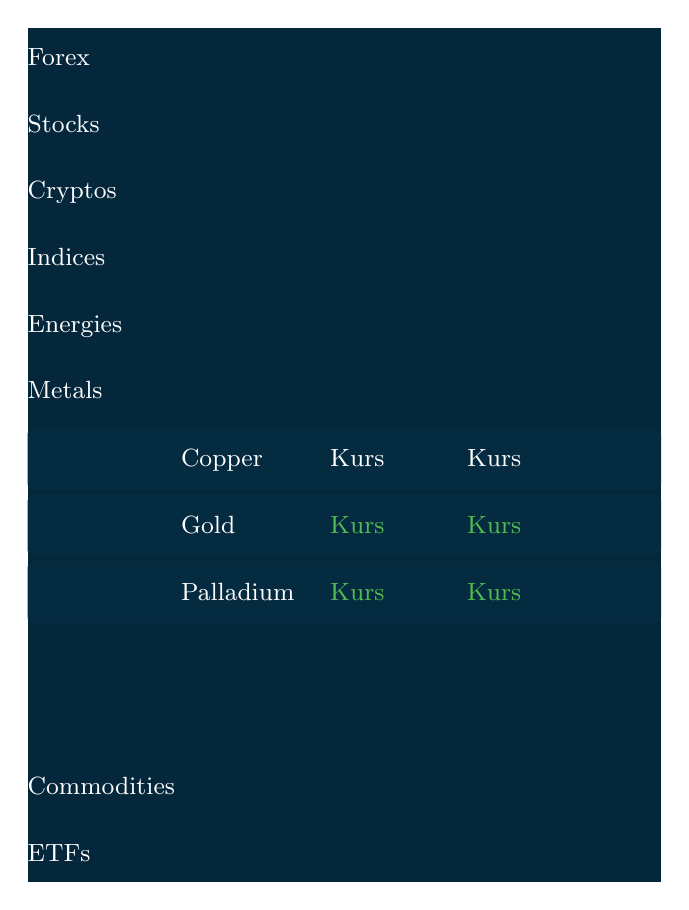
\begin{tikzpicture}[x=\px,y={(0,-\px)},font=\schrift]
  \path[use as bounding box] (0,0) rectangle (304,410);
  \fill[seite] (0,0) rectangle (304,410);
  \kategorie{0}{Forex}
  \kategorie{32}{Stocks}
  \kategorie{64}{Cryptos}
  \kategorie{96}{Indices}
  \kategorie{128}{Energies}
  \kategorie{160}{Metals}
  \instrument{192}{Copper}{white}
  \instrument{224}{Gold}{gruen}
  \instrument{256}{Palladium}{gruen}
  \kategorie{350}{Commodities}
  \kategorie{382}{ETFs}
  \ifmarken
    \marke{224+8.5+7}{1}
  \fi
\end{tikzpicture}%
\end{document}
'):
% Stil der Nummern in panel.pdf (weißer Kreis 22 px, Ziffer Inter 600 12 px in #04273C,
% Grundlinie 4 px unter der Mitte); 1 links neben dem Info-Zeichen der Zeile Gold (3 px
% Abstand, mittig zum Zeichen).
\documentclass[border=0pt]{standalone}
\usepackage{fontspec}
\usepackage{tikz}
\setmainfont{Inter}% Inter 4.0 (Paket fonts-inter), wie bar.tex
\newfontfamily\mittel{Inter Medium}%     button.quotes-ttl, font-weight 500
\newfontfamily\halbfett{Inter SemiBold}% Ziffern der Marken (wie panel.pdf)

\newlength\px \setlength\px{0.75bp}% 1 CSS-px
\newcommand\schrift{\fontsize{9bp}{10.5bp}\selectfont}% 12 px
\definecolor{seite}{RGB}{4,39,60}%      Block und Schaltflächen
% Zeile: rgba(14,80,114,0.1) über rgb(4,39,60) = (5,0; 43,1; 65,4) -> rgb(5,43,65)
\definecolor{zeile}{RGB}{5,43,65}%
\definecolor{stern}{RGB}{91,106,130}%   i.icon-star
\definecolor{info}{RGB}{34,100,134}%    i.icon-information
\definecolor{gruen}{RGB}{83,188,81}%    color-green-main
\definecolor{markenziffer}{HTML}{04273C}% Ziffer der Marken (wie panel.pdf)
% Icons als TikZ-Pfade – erzeugt von tools/icons_aus_font.py, nicht von Hand ändern.
% Schrift: 230d1684-icomoon-1-icomoon.b9abfeda36b81d3e.ttf (icomoon, Version 1.0, TrueType), sha256 951e3a5eca89112f…
% Herkunft: Webfont „icomoon“ der Plattform (icomoon.b9abfeda36b81d3e.ttf; icomoon.47a83e5a26e26197.woff hat dieselben Tabellen und Glyphen), vom Nutzer hochgeladen am 02.10.2026. Die Schriftdateien liegen NICHT im Repo (Lizenz unklar), nur diese Pfade.
% unitsPerEm 1024; Metriken hhea: Ascent 960, Descent -64.
% Box wie das <i>-Element im Browser: font-size 24px, line-height 24px
% -> Box 24 x 24 px, Ursprung unten links, y nach oben;
%    Grundlinie 1.500 px über der Boxunterkante. 1 Einheit = 1 CSS-px.
% Füllregel nonzero (wie im Browser). Farbe kommt von außen (color=…).
% Gebrauch: \begin{scope}[shift={(<x>,<y>)},x=\px,y=\px,color=<Farbe>]\iconbell\end{scope}

% U+E938 uniE938 – icon-notifications (Glocke); Vorschub 24.000 px; Umriss x 1.99–22.01, y 1.99–22.01 px; 3 Kontur(en)
\newcommand\iconbell{\fill[nonzero rule]
    (19.992,7.711) -- (22.008,7.711) -- (22.008,5.812) -- (1.992,5.812) -- (1.992,7.711) -- (4.008,7.711) -- (4.008,14.391) .. controls (4.008,15.391) and (4.211,16.359) .. (4.617,17.297) .. controls (5.023,18.234) and (5.602,19.055) .. (6.352,19.758) .. controls (7.102,20.477) and (7.965,21.031) .. (8.941,21.422) .. controls (9.918,21.812) and (10.938,22.008) .. (12,22.008) .. controls (13.062,22.008) and (14.082,21.812) .. (15.059,21.422) .. controls (16.035,21.031) and (16.898,20.477) .. (17.648,19.758) .. controls (18.398,19.055) and (18.977,18.234) .. (19.383,17.297) .. controls (19.789,16.359) and (19.992,15.391) .. (19.992,14.391) -- (19.992,7.711) -- cycle
    (18,7.711) -- (18,14.391) .. controls (18,15.141) and (17.848,15.867) .. (17.543,16.57) .. controls (17.238,17.273) and (16.805,17.891) .. (16.242,18.422) .. controls (15.68,18.953) and (15.031,19.363) .. (14.297,19.652) .. controls (13.562,19.941) and (12.797,20.086) .. (12,20.086) .. controls (11.203,20.086) and (10.438,19.941) .. (9.703,19.652) .. controls (8.969,19.363) and (8.32,18.953) .. (7.758,18.422) .. controls (7.195,17.891) and (6.762,17.273) .. (6.457,16.57) .. controls (6.152,15.867) and (6,15.141) .. (6,14.391) -- (6,7.711) -- cycle
    (9,3.891) -- (15,3.891) -- (15,1.992) -- (9,1.992) -- cycle;}

% U+E937 uniE937 – icon-settings (Zahnrad); Vorschub 24.000 px; Umriss x 2.37–21.63, y 1.99–22.01 px; 4 Kontur(en)
\newcommand\icongear{\fill[nonzero rule]
    (3.352,7.008) .. controls (3.133,7.367) and (2.941,7.742) .. (2.777,8.133) .. controls (2.613,8.523) and (2.477,8.922) .. (2.367,9.328) .. controls (2.617,9.453) and (2.844,9.609) .. (3.047,9.797) .. controls (3.25,9.984) and (3.422,10.195) .. (3.562,10.43) .. controls (3.703,10.664) and (3.812,10.914) .. (3.891,11.18) .. controls (3.969,11.445) and (4.008,11.719) .. (4.008,12) .. controls (4.008,12.281) and (3.969,12.555) .. (3.891,12.82) .. controls (3.812,13.086) and (3.703,13.336) .. (3.562,13.57) .. controls (3.422,13.805) and (3.25,14.016) .. (3.047,14.203) .. controls (2.844,14.391) and (2.617,14.547) .. (2.367,14.672) .. controls (2.586,15.484) and (2.91,16.258) .. (3.34,16.992) .. controls (3.77,17.727) and (4.281,18.398) .. (4.875,19.008) .. controls (5.094,18.852) and (5.336,18.734) .. (5.602,18.656) .. controls (5.867,18.578) and (6.141,18.531) .. (6.422,18.516) .. controls (6.703,18.516) and (6.977,18.551) .. (7.242,18.621) .. controls (7.508,18.691) and (7.758,18.797) .. (7.992,18.938) .. controls (8.242,19.062) and (8.461,19.227) .. (8.648,19.43) .. controls (8.836,19.633) and (9,19.852) .. (9.141,20.086) .. controls (9.266,20.336) and (9.359,20.594) .. (9.422,20.859) .. controls (9.484,21.125) and (9.508,21.398) .. (9.492,21.68) .. controls (10.32,21.898) and (11.156,22.008) .. (12,22.008) .. controls (12.844,22.008) and (13.68,21.898) .. (14.508,21.68) .. controls (14.492,21.398) and (14.516,21.125) .. (14.578,20.859) .. controls (14.641,20.594) and (14.734,20.336) .. (14.859,20.086) .. controls (15,19.852) and (15.164,19.633) .. (15.352,19.43) .. controls (15.539,19.227) and (15.758,19.062) .. (16.008,18.938) .. controls (16.242,18.797) and (16.492,18.691) .. (16.758,18.621) .. controls (17.023,18.551) and (17.297,18.516) .. (17.578,18.516) .. controls (17.859,18.531) and (18.133,18.578) .. (18.398,18.656) .. controls (18.664,18.734) and (18.906,18.852) .. (19.125,19.008) .. controls (19.422,18.711) and (19.699,18.395) .. (19.957,18.059) .. controls (20.215,17.723) and (20.445,17.367) .. (20.648,16.992) .. controls (20.867,16.617) and (21.059,16.238) .. (21.223,15.855) .. controls (21.387,15.473) and (21.523,15.078) .. (21.633,14.672) .. controls (21.383,14.547) and (21.156,14.391) .. (20.953,14.203) .. controls (20.75,14.016) and (20.578,13.805) .. (20.438,13.57) .. controls (20.297,13.336) and (20.188,13.086) .. (20.109,12.82) .. controls (20.031,12.555) and (19.992,12.281) .. (19.992,12) .. controls (19.992,11.719) and (20.031,11.445) .. (20.109,11.18) .. controls (20.188,10.914) and (20.297,10.664) .. (20.438,10.43) .. controls (20.578,10.195) and (20.75,9.984) .. (20.953,9.797) .. controls (21.156,9.609) and (21.383,9.453) .. (21.633,9.328) .. controls (21.414,8.516) and (21.09,7.742) .. (20.66,7.008) .. controls (20.23,6.273) and (19.719,5.602) .. (19.125,4.992) .. controls (18.906,5.148) and (18.664,5.266) .. (18.398,5.344) .. controls (18.133,5.422) and (17.859,5.469) .. (17.578,5.484) .. controls (17.297,5.484) and (17.023,5.449) .. (16.758,5.379) .. controls (16.492,5.309) and (16.242,5.203) .. (16.008,5.062) .. controls (15.758,4.938) and (15.539,4.773) .. (15.352,4.57) .. controls (15.164,4.367) and (15,4.148) .. (14.859,3.914) .. controls (14.734,3.664) and (14.641,3.406) .. (14.578,3.141) .. controls (14.516,2.875) and (14.492,2.602) .. (14.508,2.32) .. controls (13.68,2.102) and (12.844,1.992) .. (12,1.992) .. controls (11.156,1.992) and (10.32,2.102) .. (9.492,2.32) .. controls (9.508,2.602) and (9.484,2.875) .. (9.422,3.141) .. controls (9.359,3.406) and (9.266,3.664) .. (9.141,3.914) .. controls (9,4.148) and (8.836,4.367) .. (8.648,4.57) .. controls (8.461,4.773) and (8.242,4.938) .. (7.992,5.062) .. controls (7.758,5.203) and (7.508,5.309) .. (7.242,5.379) .. controls (6.977,5.449) and (6.703,5.484) .. (6.422,5.484) .. controls (6.141,5.469) and (5.867,5.422) .. (5.602,5.344) .. controls (5.336,5.266) and (5.094,5.148) .. (4.875,4.992) .. controls (4.578,5.289) and (4.301,5.605) .. (4.043,5.941) .. controls (3.785,6.277) and (3.555,6.633) .. (3.352,7.008) -- cycle
    (9,6.797) .. controls (9.531,6.5) and (9.992,6.113) .. (10.383,5.637) .. controls (10.773,5.16) and (11.062,4.625) .. (11.25,4.031) .. controls (11.5,4.016) and (11.75,4.008) .. (12,4.008) .. controls (12.25,4.008) and (12.5,4.016) .. (12.75,4.031) .. controls (12.938,4.609) and (13.227,5.141) .. (13.617,5.625) .. controls (14.008,6.109) and (14.469,6.5) .. (15,6.797) .. controls (15.531,7.109) and (16.102,7.312) .. (16.711,7.406) .. controls (17.32,7.5) and (17.922,7.484) .. (18.516,7.359) .. controls (18.672,7.562) and (18.812,7.773) .. (18.938,7.992) .. controls (19.062,8.211) and (19.172,8.438) .. (19.266,8.672) .. controls (18.859,9.125) and (18.547,9.641) .. (18.328,10.219) .. controls (18.109,10.797) and (18,11.391) .. (18,12) .. controls (18,12.625) and (18.113,13.227) .. (18.34,13.805) .. controls (18.566,14.383) and (18.875,14.891) .. (19.266,15.328) .. controls (19.172,15.562) and (19.062,15.789) .. (18.938,16.008) .. controls (18.812,16.227) and (18.672,16.438) .. (18.516,16.641) .. controls (17.922,16.516) and (17.32,16.5) .. (16.711,16.594) .. controls (16.102,16.688) and (15.531,16.891) .. (15,17.203) .. controls (14.469,17.5) and (14.008,17.887) .. (13.617,18.363) .. controls (13.227,18.84) and (12.938,19.375) .. (12.75,19.969) .. controls (12.5,19.984) and (12.25,19.992) .. (12,19.992) .. controls (11.75,19.992) and (11.5,19.984) .. (11.25,19.969) .. controls (11.062,19.391) and (10.773,18.859) .. (10.383,18.375) .. controls (9.992,17.891) and (9.531,17.5) .. (9,17.203) .. controls (8.469,16.891) and (7.898,16.688) .. (7.289,16.594) .. controls (6.68,16.5) and (6.078,16.516) .. (5.484,16.641) .. controls (5.328,16.438) and (5.188,16.227) .. (5.062,16.008) .. controls (4.938,15.789) and (4.828,15.562) .. (4.734,15.328) .. controls (5.141,14.875) and (5.453,14.359) .. (5.672,13.781) .. controls (5.891,13.203) and (6,12.609) .. (6,12) .. controls (6,11.375) and (5.887,10.773) .. (5.66,10.195) .. controls (5.434,9.617) and (5.125,9.109) .. (4.734,8.672) .. controls (4.828,8.438) and (4.938,8.211) .. (5.062,7.992) .. controls (5.188,7.773) and (5.328,7.562) .. (5.484,7.359) .. controls (6.078,7.484) and (6.68,7.5) .. (7.289,7.406) .. controls (7.898,7.312) and (8.469,7.109) .. (9,6.797) -- cycle
    (12,9) .. controls (11.609,9) and (11.227,9.074) .. (10.852,9.223) .. controls (10.477,9.371) and (10.148,9.586) .. (9.867,9.867) .. controls (9.586,10.148) and (9.371,10.477) .. (9.223,10.852) .. controls (9.074,11.227) and (9,11.609) .. (9,12) .. controls (9,12.391) and (9.074,12.773) .. (9.223,13.148) .. controls (9.371,13.523) and (9.586,13.852) .. (9.867,14.133) .. controls (10.148,14.414) and (10.477,14.629) .. (10.852,14.777) .. controls (11.227,14.926) and (11.609,15) .. (12,15) .. controls (12.391,15) and (12.773,14.926) .. (13.148,14.777) .. controls (13.523,14.629) and (13.852,14.414) .. (14.133,14.133) .. controls (14.414,13.852) and (14.629,13.523) .. (14.777,13.148) .. controls (14.926,12.773) and (15,12.391) .. (15,12) .. controls (15,11.609) and (14.926,11.227) .. (14.777,10.852) .. controls (14.629,10.477) and (14.414,10.148) .. (14.133,9.867) .. controls (13.852,9.586) and (13.523,9.371) .. (13.148,9.223) .. controls (12.773,9.074) and (12.391,9) .. (12,9) -- cycle
    (12,10.992) .. controls (12.125,10.992) and (12.25,11.02) .. (12.375,11.074) .. controls (12.5,11.129) and (12.609,11.203) .. (12.703,11.297) .. controls (12.797,11.391) and (12.871,11.5) .. (12.926,11.625) .. controls (12.98,11.75) and (13.008,11.875) .. (13.008,12) .. controls (13.008,12.125) and (12.98,12.25) .. (12.926,12.375) .. controls (12.871,12.5) and (12.797,12.609) .. (12.703,12.703) .. controls (12.609,12.797) and (12.5,12.871) .. (12.375,12.926) .. controls (12.25,12.98) and (12.125,13.008) .. (12,13.008) .. controls (11.875,13.008) and (11.75,12.98) .. (11.625,12.926) .. controls (11.5,12.871) and (11.391,12.797) .. (11.297,12.703) .. controls (11.203,12.609) and (11.129,12.5) .. (11.074,12.375) .. controls (11.02,12.25) and (10.992,12.125) .. (10.992,12) .. controls (10.992,11.875) and (11.02,11.75) .. (11.074,11.625) .. controls (11.129,11.5) and (11.203,11.391) .. (11.297,11.297) .. controls (11.391,11.203) and (11.5,11.129) .. (11.625,11.074) .. controls (11.75,11.02) and (11.875,10.992) .. (12,10.992) -- cycle;}

% U+E90C uniE90C – icon-orders (Liste mit Plus); Vorschub 24.000 px; Umriss x 3.00–21.00, y 1.01–19.99 px; 4 Kontur(en)
\newcommand\iconorders{\fill[nonzero rule]
    (18,9) -- (18,6) -- (21,6) -- (21,4.008) -- (18,4.008) -- (18,1.008) -- (16.008,1.008) -- (16.008,4.008) -- (13.008,4.008) -- (13.008,6) -- (16.008,6) -- (16.008,9) -- cycle
    (10.992,6) -- (10.992,4.008) -- (3,4.008) -- (3,6) -- cycle
    (21,13.008) -- (21,10.992) -- (3,10.992) -- (3,13.008) -- (21,13.008) -- cycle
    (21,19.992) -- (21,18) -- (3,18) -- (3,19.992) -- cycle;}

% U+E93A uniE93A – icon-information (Kreis mit i); Vorschub 24.000 px; Umriss x 1.99–22.01, y 1.99–22.01 px; 4 Kontur(en)
\newcommand\iconinfo{\fill[nonzero rule]
    (12,1.992) .. controls (10.625,1.992) and (9.328,2.258) .. (8.109,2.789) .. controls (6.891,3.305) and (5.828,4.016) .. (4.922,4.922) .. controls (4.016,5.828) and (3.305,6.891) .. (2.789,8.109) .. controls (2.258,9.328) and (1.992,10.625) .. (1.992,12) .. controls (1.992,13.375) and (2.258,14.672) .. (2.789,15.891) .. controls (3.305,17.109) and (4.016,18.172) .. (4.922,19.078) .. controls (5.828,19.984) and (6.891,20.695) .. (8.109,21.211) .. controls (9.328,21.742) and (10.625,22.008) .. (12,22.008) .. controls (13.375,22.008) and (14.672,21.742) .. (15.891,21.211) .. controls (17.109,20.695) and (18.172,19.984) .. (19.078,19.078) .. controls (19.984,18.172) and (20.695,17.109) .. (21.211,15.891) .. controls (21.742,14.672) and (22.008,13.375) .. (22.008,12) .. controls (22.008,10.625) and (21.742,9.328) .. (21.211,8.109) .. controls (20.695,6.891) and (19.984,5.828) .. (19.078,4.922) .. controls (18.172,4.016) and (17.109,3.305) .. (15.891,2.789) .. controls (14.672,2.258) and (13.375,1.992) .. (12,1.992) -- cycle
    (12,4.008) .. controls (13.062,4.008) and (14.082,4.211) .. (15.059,4.617) .. controls (16.035,5.023) and (16.898,5.602) .. (17.648,6.352) .. controls (18.398,7.102) and (18.977,7.965) .. (19.383,8.941) .. controls (19.789,9.918) and (19.992,10.938) .. (19.992,12) .. controls (19.992,13.062) and (19.789,14.082) .. (19.383,15.059) .. controls (18.977,16.035) and (18.398,16.898) .. (17.648,17.648) .. controls (16.898,18.398) and (16.035,18.977) .. (15.059,19.383) .. controls (14.082,19.789) and (13.062,19.992) .. (12,19.992) .. controls (10.938,19.992) and (9.918,19.789) .. (8.941,19.383) .. controls (7.965,18.977) and (7.102,18.398) .. (6.352,17.648) .. controls (5.602,16.898) and (5.023,16.035) .. (4.617,15.059) .. controls (4.211,14.082) and (4.008,13.062) .. (4.008,12) .. controls (4.008,10.938) and (4.211,9.918) .. (4.617,8.941) .. controls (5.023,7.965) and (5.602,7.102) .. (6.352,6.352) .. controls (7.102,5.602) and (7.965,5.023) .. (8.941,4.617) .. controls (9.918,4.211) and (10.938,4.008) .. (12,4.008) -- cycle
    (10.992,16.992) -- (13.008,16.992) -- (13.008,15) -- (10.992,15) -- (10.992,16.992) -- cycle
    (10.992,13.008) -- (13.008,13.008) -- (13.008,7.008) -- (10.992,7.008) -- (10.992,13.008) -- cycle;}


\newif\ifmarken \markentrue
\ifdefined\ohnemarken \markenfalse\fi

% \kategorie{<y>}{<Name>}
\newcommand\kategorie[2]{%
  \node[anchor=base west,inner sep=0,outer sep=0,text=white,font=\schrift\mittel]
    at (0,#1+18.2) {#2};}

% \icon{<x>}{<y Oberkante>}{<Farbe>}{<Icon>}: Box 14 x 14 px (icons.tikz: 24 px, y nach oben)
\newcommand\icon[4]{%
  \begin{scope}[shift={(#1,#2+14)},x=0.4375bp,y=0.4375bp,color=#3]#4\end{scope}}% 14/24 px

% \instrument{<y>}{<Name>}{<Farbe der Kurse>}
\newcommand\instrument[3]{%
  \fill[zeile,rounded corners=3\px] (0,#1) rectangle (304,#1+30);
  \ifdefined\iconstar \icon{8}{#1+8}{stern}{\iconstar}\fi
  \node[anchor=base west,inner sep=0,outer sep=0,text=white] at (73.6,#1+18.8) {#2};
  \node[anchor=base west,inner sep=0,outer sep=0,text=#3] at (145.2,#1+18.8) {Kurs};
  \node[anchor=base west,inner sep=0,outer sep=0,text=#3] at (210.9,#1+18.8) {Kurs};
  \icon{278.6}{#1+8.5}{info}{\iconinfo}}

% \marke{<y Mitte>}{<Nummer>}: Kreis 22 px, 3 px links vor dem Info-Zeichen (x 278,6)
\newcommand\marke[2]{%
  \fill[white] (264.6,#1) circle[radius=11];
  \node[anchor=base,inner sep=0,outer sep=0,text=markenziffer,
    font=\schrift\halbfett] at (264.6,#1+4) {#2};}

\begin{document}%
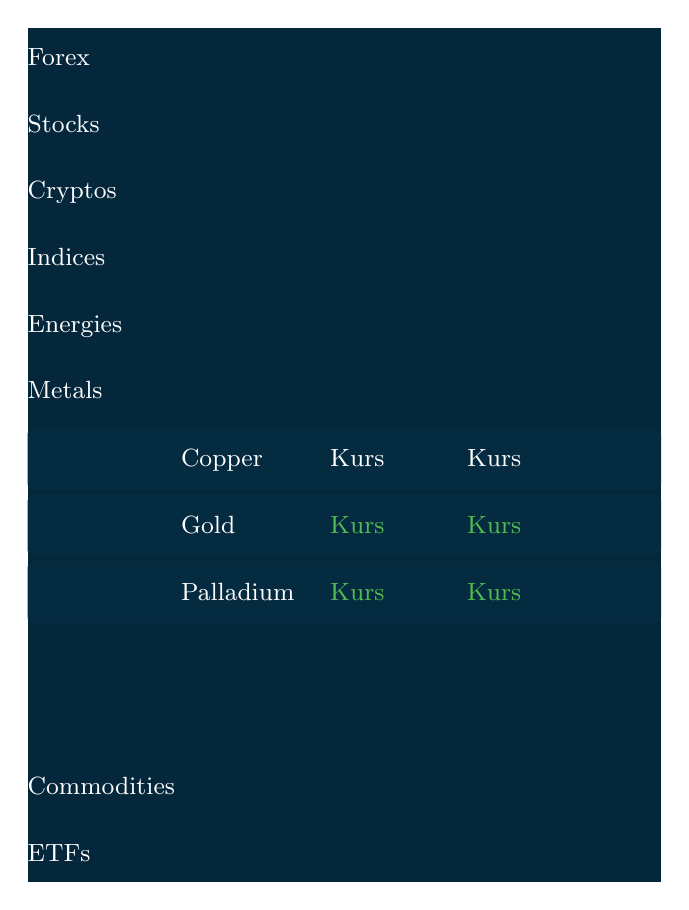
\begin{tikzpicture}[x=\px,y={(0,-\px)},font=\schrift]
  \path[use as bounding box] (0,0) rectangle (304,410);
  \fill[seite] (0,0) rectangle (304,410);
  \kategorie{0}{Forex}
  \kategorie{32}{Stocks}
  \kategorie{64}{Cryptos}
  \kategorie{96}{Indices}
  \kategorie{128}{Energies}
  \kategorie{160}{Metals}
  \instrument{192}{Copper}{white}
  \instrument{224}{Gold}{gruen}
  \instrument{256}{Palladium}{gruen}
  \kategorie{350}{Commodities}
  \kategorie{382}{ETFs}
  \ifmarken
    \marke{224+8.5+7}{1}
  \fi
\end{tikzpicture}%
\end{document}
'):
% Stil der Nummern in panel.pdf (weißer Kreis 22 px, Ziffer Inter 600 12 px in #04273C,
% Grundlinie 4 px unter der Mitte); 1 links neben dem Info-Zeichen der Zeile Gold (3 px
% Abstand, mittig zum Zeichen).
\documentclass[border=0pt]{standalone}
\usepackage{fontspec}
\usepackage{tikz}
\setmainfont{Inter}% Inter 4.0 (Paket fonts-inter), wie bar.tex
\newfontfamily\mittel{Inter Medium}%     button.quotes-ttl, font-weight 500
\newfontfamily\halbfett{Inter SemiBold}% Ziffern der Marken (wie panel.pdf)

\newlength\px \setlength\px{0.75bp}% 1 CSS-px
\newcommand\schrift{\fontsize{9bp}{10.5bp}\selectfont}% 12 px
\definecolor{seite}{RGB}{4,39,60}%      Block und Schaltflächen
% Zeile: rgba(14,80,114,0.1) über rgb(4,39,60) = (5,0; 43,1; 65,4) -> rgb(5,43,65)
\definecolor{zeile}{RGB}{5,43,65}%
\definecolor{stern}{RGB}{91,106,130}%   i.icon-star
\definecolor{info}{RGB}{34,100,134}%    i.icon-information
\definecolor{gruen}{RGB}{83,188,81}%    color-green-main
\definecolor{markenziffer}{HTML}{04273C}% Ziffer der Marken (wie panel.pdf)
% Icons als TikZ-Pfade – erzeugt von tools/icons_aus_font.py, nicht von Hand ändern.
% Schrift: 230d1684-icomoon-1-icomoon.b9abfeda36b81d3e.ttf (icomoon, Version 1.0, TrueType), sha256 951e3a5eca89112f…
% Herkunft: Webfont „icomoon“ der Plattform (icomoon.b9abfeda36b81d3e.ttf; icomoon.47a83e5a26e26197.woff hat dieselben Tabellen und Glyphen), vom Nutzer hochgeladen am 02.10.2026. Die Schriftdateien liegen NICHT im Repo (Lizenz unklar), nur diese Pfade.
% unitsPerEm 1024; Metriken hhea: Ascent 960, Descent -64.
% Box wie das <i>-Element im Browser: font-size 24px, line-height 24px
% -> Box 24 x 24 px, Ursprung unten links, y nach oben;
%    Grundlinie 1.500 px über der Boxunterkante. 1 Einheit = 1 CSS-px.
% Füllregel nonzero (wie im Browser). Farbe kommt von außen (color=…).
% Gebrauch: \begin{scope}[shift={(<x>,<y>)},x=\px,y=\px,color=<Farbe>]\iconbell\end{scope}

% U+E938 uniE938 – icon-notifications (Glocke); Vorschub 24.000 px; Umriss x 1.99–22.01, y 1.99–22.01 px; 3 Kontur(en)
\newcommand\iconbell{\fill[nonzero rule]
    (19.992,7.711) -- (22.008,7.711) -- (22.008,5.812) -- (1.992,5.812) -- (1.992,7.711) -- (4.008,7.711) -- (4.008,14.391) .. controls (4.008,15.391) and (4.211,16.359) .. (4.617,17.297) .. controls (5.023,18.234) and (5.602,19.055) .. (6.352,19.758) .. controls (7.102,20.477) and (7.965,21.031) .. (8.941,21.422) .. controls (9.918,21.812) and (10.938,22.008) .. (12,22.008) .. controls (13.062,22.008) and (14.082,21.812) .. (15.059,21.422) .. controls (16.035,21.031) and (16.898,20.477) .. (17.648,19.758) .. controls (18.398,19.055) and (18.977,18.234) .. (19.383,17.297) .. controls (19.789,16.359) and (19.992,15.391) .. (19.992,14.391) -- (19.992,7.711) -- cycle
    (18,7.711) -- (18,14.391) .. controls (18,15.141) and (17.848,15.867) .. (17.543,16.57) .. controls (17.238,17.273) and (16.805,17.891) .. (16.242,18.422) .. controls (15.68,18.953) and (15.031,19.363) .. (14.297,19.652) .. controls (13.562,19.941) and (12.797,20.086) .. (12,20.086) .. controls (11.203,20.086) and (10.438,19.941) .. (9.703,19.652) .. controls (8.969,19.363) and (8.32,18.953) .. (7.758,18.422) .. controls (7.195,17.891) and (6.762,17.273) .. (6.457,16.57) .. controls (6.152,15.867) and (6,15.141) .. (6,14.391) -- (6,7.711) -- cycle
    (9,3.891) -- (15,3.891) -- (15,1.992) -- (9,1.992) -- cycle;}

% U+E937 uniE937 – icon-settings (Zahnrad); Vorschub 24.000 px; Umriss x 2.37–21.63, y 1.99–22.01 px; 4 Kontur(en)
\newcommand\icongear{\fill[nonzero rule]
    (3.352,7.008) .. controls (3.133,7.367) and (2.941,7.742) .. (2.777,8.133) .. controls (2.613,8.523) and (2.477,8.922) .. (2.367,9.328) .. controls (2.617,9.453) and (2.844,9.609) .. (3.047,9.797) .. controls (3.25,9.984) and (3.422,10.195) .. (3.562,10.43) .. controls (3.703,10.664) and (3.812,10.914) .. (3.891,11.18) .. controls (3.969,11.445) and (4.008,11.719) .. (4.008,12) .. controls (4.008,12.281) and (3.969,12.555) .. (3.891,12.82) .. controls (3.812,13.086) and (3.703,13.336) .. (3.562,13.57) .. controls (3.422,13.805) and (3.25,14.016) .. (3.047,14.203) .. controls (2.844,14.391) and (2.617,14.547) .. (2.367,14.672) .. controls (2.586,15.484) and (2.91,16.258) .. (3.34,16.992) .. controls (3.77,17.727) and (4.281,18.398) .. (4.875,19.008) .. controls (5.094,18.852) and (5.336,18.734) .. (5.602,18.656) .. controls (5.867,18.578) and (6.141,18.531) .. (6.422,18.516) .. controls (6.703,18.516) and (6.977,18.551) .. (7.242,18.621) .. controls (7.508,18.691) and (7.758,18.797) .. (7.992,18.938) .. controls (8.242,19.062) and (8.461,19.227) .. (8.648,19.43) .. controls (8.836,19.633) and (9,19.852) .. (9.141,20.086) .. controls (9.266,20.336) and (9.359,20.594) .. (9.422,20.859) .. controls (9.484,21.125) and (9.508,21.398) .. (9.492,21.68) .. controls (10.32,21.898) and (11.156,22.008) .. (12,22.008) .. controls (12.844,22.008) and (13.68,21.898) .. (14.508,21.68) .. controls (14.492,21.398) and (14.516,21.125) .. (14.578,20.859) .. controls (14.641,20.594) and (14.734,20.336) .. (14.859,20.086) .. controls (15,19.852) and (15.164,19.633) .. (15.352,19.43) .. controls (15.539,19.227) and (15.758,19.062) .. (16.008,18.938) .. controls (16.242,18.797) and (16.492,18.691) .. (16.758,18.621) .. controls (17.023,18.551) and (17.297,18.516) .. (17.578,18.516) .. controls (17.859,18.531) and (18.133,18.578) .. (18.398,18.656) .. controls (18.664,18.734) and (18.906,18.852) .. (19.125,19.008) .. controls (19.422,18.711) and (19.699,18.395) .. (19.957,18.059) .. controls (20.215,17.723) and (20.445,17.367) .. (20.648,16.992) .. controls (20.867,16.617) and (21.059,16.238) .. (21.223,15.855) .. controls (21.387,15.473) and (21.523,15.078) .. (21.633,14.672) .. controls (21.383,14.547) and (21.156,14.391) .. (20.953,14.203) .. controls (20.75,14.016) and (20.578,13.805) .. (20.438,13.57) .. controls (20.297,13.336) and (20.188,13.086) .. (20.109,12.82) .. controls (20.031,12.555) and (19.992,12.281) .. (19.992,12) .. controls (19.992,11.719) and (20.031,11.445) .. (20.109,11.18) .. controls (20.188,10.914) and (20.297,10.664) .. (20.438,10.43) .. controls (20.578,10.195) and (20.75,9.984) .. (20.953,9.797) .. controls (21.156,9.609) and (21.383,9.453) .. (21.633,9.328) .. controls (21.414,8.516) and (21.09,7.742) .. (20.66,7.008) .. controls (20.23,6.273) and (19.719,5.602) .. (19.125,4.992) .. controls (18.906,5.148) and (18.664,5.266) .. (18.398,5.344) .. controls (18.133,5.422) and (17.859,5.469) .. (17.578,5.484) .. controls (17.297,5.484) and (17.023,5.449) .. (16.758,5.379) .. controls (16.492,5.309) and (16.242,5.203) .. (16.008,5.062) .. controls (15.758,4.938) and (15.539,4.773) .. (15.352,4.57) .. controls (15.164,4.367) and (15,4.148) .. (14.859,3.914) .. controls (14.734,3.664) and (14.641,3.406) .. (14.578,3.141) .. controls (14.516,2.875) and (14.492,2.602) .. (14.508,2.32) .. controls (13.68,2.102) and (12.844,1.992) .. (12,1.992) .. controls (11.156,1.992) and (10.32,2.102) .. (9.492,2.32) .. controls (9.508,2.602) and (9.484,2.875) .. (9.422,3.141) .. controls (9.359,3.406) and (9.266,3.664) .. (9.141,3.914) .. controls (9,4.148) and (8.836,4.367) .. (8.648,4.57) .. controls (8.461,4.773) and (8.242,4.938) .. (7.992,5.062) .. controls (7.758,5.203) and (7.508,5.309) .. (7.242,5.379) .. controls (6.977,5.449) and (6.703,5.484) .. (6.422,5.484) .. controls (6.141,5.469) and (5.867,5.422) .. (5.602,5.344) .. controls (5.336,5.266) and (5.094,5.148) .. (4.875,4.992) .. controls (4.578,5.289) and (4.301,5.605) .. (4.043,5.941) .. controls (3.785,6.277) and (3.555,6.633) .. (3.352,7.008) -- cycle
    (9,6.797) .. controls (9.531,6.5) and (9.992,6.113) .. (10.383,5.637) .. controls (10.773,5.16) and (11.062,4.625) .. (11.25,4.031) .. controls (11.5,4.016) and (11.75,4.008) .. (12,4.008) .. controls (12.25,4.008) and (12.5,4.016) .. (12.75,4.031) .. controls (12.938,4.609) and (13.227,5.141) .. (13.617,5.625) .. controls (14.008,6.109) and (14.469,6.5) .. (15,6.797) .. controls (15.531,7.109) and (16.102,7.312) .. (16.711,7.406) .. controls (17.32,7.5) and (17.922,7.484) .. (18.516,7.359) .. controls (18.672,7.562) and (18.812,7.773) .. (18.938,7.992) .. controls (19.062,8.211) and (19.172,8.438) .. (19.266,8.672) .. controls (18.859,9.125) and (18.547,9.641) .. (18.328,10.219) .. controls (18.109,10.797) and (18,11.391) .. (18,12) .. controls (18,12.625) and (18.113,13.227) .. (18.34,13.805) .. controls (18.566,14.383) and (18.875,14.891) .. (19.266,15.328) .. controls (19.172,15.562) and (19.062,15.789) .. (18.938,16.008) .. controls (18.812,16.227) and (18.672,16.438) .. (18.516,16.641) .. controls (17.922,16.516) and (17.32,16.5) .. (16.711,16.594) .. controls (16.102,16.688) and (15.531,16.891) .. (15,17.203) .. controls (14.469,17.5) and (14.008,17.887) .. (13.617,18.363) .. controls (13.227,18.84) and (12.938,19.375) .. (12.75,19.969) .. controls (12.5,19.984) and (12.25,19.992) .. (12,19.992) .. controls (11.75,19.992) and (11.5,19.984) .. (11.25,19.969) .. controls (11.062,19.391) and (10.773,18.859) .. (10.383,18.375) .. controls (9.992,17.891) and (9.531,17.5) .. (9,17.203) .. controls (8.469,16.891) and (7.898,16.688) .. (7.289,16.594) .. controls (6.68,16.5) and (6.078,16.516) .. (5.484,16.641) .. controls (5.328,16.438) and (5.188,16.227) .. (5.062,16.008) .. controls (4.938,15.789) and (4.828,15.562) .. (4.734,15.328) .. controls (5.141,14.875) and (5.453,14.359) .. (5.672,13.781) .. controls (5.891,13.203) and (6,12.609) .. (6,12) .. controls (6,11.375) and (5.887,10.773) .. (5.66,10.195) .. controls (5.434,9.617) and (5.125,9.109) .. (4.734,8.672) .. controls (4.828,8.438) and (4.938,8.211) .. (5.062,7.992) .. controls (5.188,7.773) and (5.328,7.562) .. (5.484,7.359) .. controls (6.078,7.484) and (6.68,7.5) .. (7.289,7.406) .. controls (7.898,7.312) and (8.469,7.109) .. (9,6.797) -- cycle
    (12,9) .. controls (11.609,9) and (11.227,9.074) .. (10.852,9.223) .. controls (10.477,9.371) and (10.148,9.586) .. (9.867,9.867) .. controls (9.586,10.148) and (9.371,10.477) .. (9.223,10.852) .. controls (9.074,11.227) and (9,11.609) .. (9,12) .. controls (9,12.391) and (9.074,12.773) .. (9.223,13.148) .. controls (9.371,13.523) and (9.586,13.852) .. (9.867,14.133) .. controls (10.148,14.414) and (10.477,14.629) .. (10.852,14.777) .. controls (11.227,14.926) and (11.609,15) .. (12,15) .. controls (12.391,15) and (12.773,14.926) .. (13.148,14.777) .. controls (13.523,14.629) and (13.852,14.414) .. (14.133,14.133) .. controls (14.414,13.852) and (14.629,13.523) .. (14.777,13.148) .. controls (14.926,12.773) and (15,12.391) .. (15,12) .. controls (15,11.609) and (14.926,11.227) .. (14.777,10.852) .. controls (14.629,10.477) and (14.414,10.148) .. (14.133,9.867) .. controls (13.852,9.586) and (13.523,9.371) .. (13.148,9.223) .. controls (12.773,9.074) and (12.391,9) .. (12,9) -- cycle
    (12,10.992) .. controls (12.125,10.992) and (12.25,11.02) .. (12.375,11.074) .. controls (12.5,11.129) and (12.609,11.203) .. (12.703,11.297) .. controls (12.797,11.391) and (12.871,11.5) .. (12.926,11.625) .. controls (12.98,11.75) and (13.008,11.875) .. (13.008,12) .. controls (13.008,12.125) and (12.98,12.25) .. (12.926,12.375) .. controls (12.871,12.5) and (12.797,12.609) .. (12.703,12.703) .. controls (12.609,12.797) and (12.5,12.871) .. (12.375,12.926) .. controls (12.25,12.98) and (12.125,13.008) .. (12,13.008) .. controls (11.875,13.008) and (11.75,12.98) .. (11.625,12.926) .. controls (11.5,12.871) and (11.391,12.797) .. (11.297,12.703) .. controls (11.203,12.609) and (11.129,12.5) .. (11.074,12.375) .. controls (11.02,12.25) and (10.992,12.125) .. (10.992,12) .. controls (10.992,11.875) and (11.02,11.75) .. (11.074,11.625) .. controls (11.129,11.5) and (11.203,11.391) .. (11.297,11.297) .. controls (11.391,11.203) and (11.5,11.129) .. (11.625,11.074) .. controls (11.75,11.02) and (11.875,10.992) .. (12,10.992) -- cycle;}

% U+E90C uniE90C – icon-orders (Liste mit Plus); Vorschub 24.000 px; Umriss x 3.00–21.00, y 1.01–19.99 px; 4 Kontur(en)
\newcommand\iconorders{\fill[nonzero rule]
    (18,9) -- (18,6) -- (21,6) -- (21,4.008) -- (18,4.008) -- (18,1.008) -- (16.008,1.008) -- (16.008,4.008) -- (13.008,4.008) -- (13.008,6) -- (16.008,6) -- (16.008,9) -- cycle
    (10.992,6) -- (10.992,4.008) -- (3,4.008) -- (3,6) -- cycle
    (21,13.008) -- (21,10.992) -- (3,10.992) -- (3,13.008) -- (21,13.008) -- cycle
    (21,19.992) -- (21,18) -- (3,18) -- (3,19.992) -- cycle;}

% U+E93A uniE93A – icon-information (Kreis mit i); Vorschub 24.000 px; Umriss x 1.99–22.01, y 1.99–22.01 px; 4 Kontur(en)
\newcommand\iconinfo{\fill[nonzero rule]
    (12,1.992) .. controls (10.625,1.992) and (9.328,2.258) .. (8.109,2.789) .. controls (6.891,3.305) and (5.828,4.016) .. (4.922,4.922) .. controls (4.016,5.828) and (3.305,6.891) .. (2.789,8.109) .. controls (2.258,9.328) and (1.992,10.625) .. (1.992,12) .. controls (1.992,13.375) and (2.258,14.672) .. (2.789,15.891) .. controls (3.305,17.109) and (4.016,18.172) .. (4.922,19.078) .. controls (5.828,19.984) and (6.891,20.695) .. (8.109,21.211) .. controls (9.328,21.742) and (10.625,22.008) .. (12,22.008) .. controls (13.375,22.008) and (14.672,21.742) .. (15.891,21.211) .. controls (17.109,20.695) and (18.172,19.984) .. (19.078,19.078) .. controls (19.984,18.172) and (20.695,17.109) .. (21.211,15.891) .. controls (21.742,14.672) and (22.008,13.375) .. (22.008,12) .. controls (22.008,10.625) and (21.742,9.328) .. (21.211,8.109) .. controls (20.695,6.891) and (19.984,5.828) .. (19.078,4.922) .. controls (18.172,4.016) and (17.109,3.305) .. (15.891,2.789) .. controls (14.672,2.258) and (13.375,1.992) .. (12,1.992) -- cycle
    (12,4.008) .. controls (13.062,4.008) and (14.082,4.211) .. (15.059,4.617) .. controls (16.035,5.023) and (16.898,5.602) .. (17.648,6.352) .. controls (18.398,7.102) and (18.977,7.965) .. (19.383,8.941) .. controls (19.789,9.918) and (19.992,10.938) .. (19.992,12) .. controls (19.992,13.062) and (19.789,14.082) .. (19.383,15.059) .. controls (18.977,16.035) and (18.398,16.898) .. (17.648,17.648) .. controls (16.898,18.398) and (16.035,18.977) .. (15.059,19.383) .. controls (14.082,19.789) and (13.062,19.992) .. (12,19.992) .. controls (10.938,19.992) and (9.918,19.789) .. (8.941,19.383) .. controls (7.965,18.977) and (7.102,18.398) .. (6.352,17.648) .. controls (5.602,16.898) and (5.023,16.035) .. (4.617,15.059) .. controls (4.211,14.082) and (4.008,13.062) .. (4.008,12) .. controls (4.008,10.938) and (4.211,9.918) .. (4.617,8.941) .. controls (5.023,7.965) and (5.602,7.102) .. (6.352,6.352) .. controls (7.102,5.602) and (7.965,5.023) .. (8.941,4.617) .. controls (9.918,4.211) and (10.938,4.008) .. (12,4.008) -- cycle
    (10.992,16.992) -- (13.008,16.992) -- (13.008,15) -- (10.992,15) -- (10.992,16.992) -- cycle
    (10.992,13.008) -- (13.008,13.008) -- (13.008,7.008) -- (10.992,7.008) -- (10.992,13.008) -- cycle;}


\newif\ifmarken \markentrue
\ifdefined\ohnemarken \markenfalse\fi

% \kategorie{<y>}{<Name>}
\newcommand\kategorie[2]{%
  \node[anchor=base west,inner sep=0,outer sep=0,text=white,font=\schrift\mittel]
    at (0,#1+18.2) {#2};}

% \icon{<x>}{<y Oberkante>}{<Farbe>}{<Icon>}: Box 14 x 14 px (icons.tikz: 24 px, y nach oben)
\newcommand\icon[4]{%
  \begin{scope}[shift={(#1,#2+14)},x=0.4375bp,y=0.4375bp,color=#3]#4\end{scope}}% 14/24 px

% \instrument{<y>}{<Name>}{<Farbe der Kurse>}
\newcommand\instrument[3]{%
  \fill[zeile,rounded corners=3\px] (0,#1) rectangle (304,#1+30);
  \ifdefined\iconstar \icon{8}{#1+8}{stern}{\iconstar}\fi
  \node[anchor=base west,inner sep=0,outer sep=0,text=white] at (73.6,#1+18.8) {#2};
  \node[anchor=base west,inner sep=0,outer sep=0,text=#3] at (145.2,#1+18.8) {Kurs};
  \node[anchor=base west,inner sep=0,outer sep=0,text=#3] at (210.9,#1+18.8) {Kurs};
  \icon{278.6}{#1+8.5}{info}{\iconinfo}}

% \marke{<y Mitte>}{<Nummer>}: Kreis 22 px, 3 px links vor dem Info-Zeichen (x 278,6)
\newcommand\marke[2]{%
  \fill[white] (264.6,#1) circle[radius=11];
  \node[anchor=base,inner sep=0,outer sep=0,text=markenziffer,
    font=\schrift\halbfett] at (264.6,#1+4) {#2};}

\begin{document}%
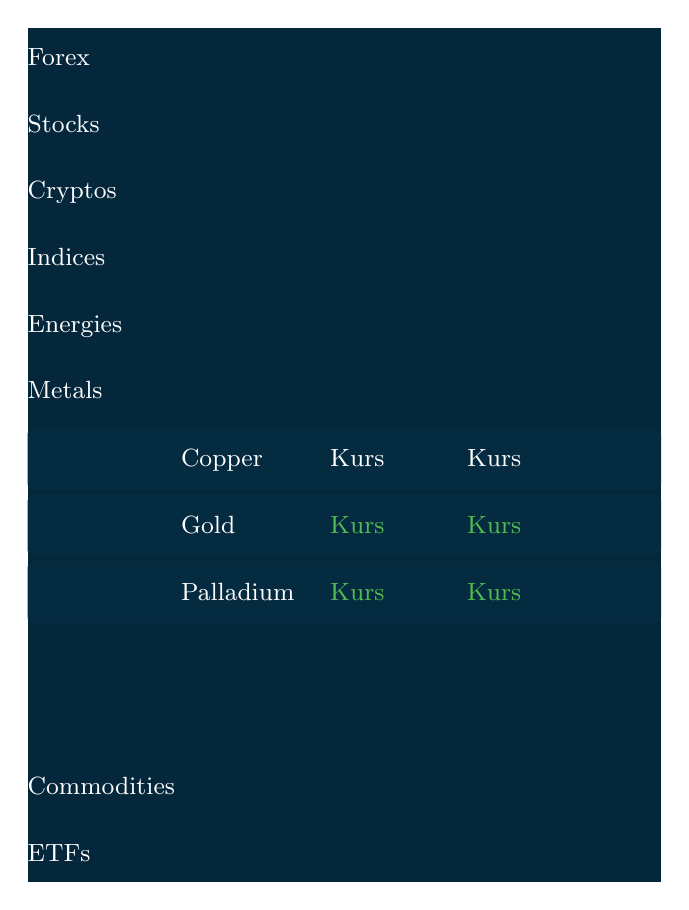
\begin{tikzpicture}[x=\px,y={(0,-\px)},font=\schrift]
  \path[use as bounding box] (0,0) rectangle (304,410);
  \fill[seite] (0,0) rectangle (304,410);
  \kategorie{0}{Forex}
  \kategorie{32}{Stocks}
  \kategorie{64}{Cryptos}
  \kategorie{96}{Indices}
  \kategorie{128}{Energies}
  \kategorie{160}{Metals}
  \instrument{192}{Copper}{white}
  \instrument{224}{Gold}{gruen}
  \instrument{256}{Palladium}{gruen}
  \kategorie{350}{Commodities}
  \kategorie{382}{ETFs}
  \ifmarken
    \marke{224+8.5+7}{1}
  \fi
\end{tikzpicture}%
\end{document}
